\chapter{RFP Equilibrium}

The success of electromagnetic containment systems depends on the ability to maintain the plasma in equilibrium in the presence of small perturbations
that could compromise its stability. In Tokamak and RFP type experiments, the instabilities that produce macroscopic effects are described, in their simplest form, by the plasma fluid model MHD ( magnetohydrodynamic model ). 
We abandon the kinetic description of the single particle to consider the set of charges, thinking of the plasma as a fluid: the dimensions of the survey region are much greater than the Debye length and the Larmor radius. Therefore, a discrete system with separate charges is no longer observed.

\subsection{Single fluid magnetohydrodynamic equilibrium}

In the MHD model the equations of classical electromagnetism are combined with those of the fluid motion. Typically the analysis of fluid plasma involves the generalized movements of each ionic species; however, for simplicity it is possible to consider each pair of values relating to ions and electrons in a single parameter and thus obtain a single fluid trend. Moreover, remembering that for fusion gases there is almost neutral charge $n_i = n_e$ the charge density term $\rho = e(n_i - n_e)$ can be omitted. The relevant quantities are thus:
\begin{itemize}
    \item the mass density of the fluid
    \begin{equation}
        \rho_m = n_e m_e + n_i m_i
    \end{equation}
    \item the mean current density per unit volume
    \begin{equation}
        \mean{J} = e(n_i \mean{v_i} - n_e \mean{v_e})
    \end{equation}
    \item the fluid pressure
    \begin{equation}
        p \approx n_e k T_e + n_i k T_i
    \end{equation}
\end{itemize}
With this variables the fluid equations and the conservation of moment and mass can be defined:
\begin{align}
    \pdv{\rho_m}{t} + \nabla \cdot (\rho_m \Vec{v}) &= 0 \\
    \rho_m \left( \pdv{\Vec{v}}{t} + \Vec{v} \cdot \nabla \Vec{v} \right) &= \Vec{J} \times \Vec{B} - \nabla p
 \end{align}
where the electromagnetic interaction can be added with the Maxwell and Ohm relations:
\begin{align}
    \nabla \times \Vec{E} &= - \pdv{\Vec{B}}{t} \label{eq:faraday} \\
    \nabla \times \Vec{B} &= \mu_0 \Vec{J} \label{eq:ampere} \\
    \nabla \cdot \Vec{B}  &= 0 \\
    \nabla \cdot \Vec{E}  &= 0 \\
    \Vec{E} + \Vec{v} \times \Vec{B} &= \eta \Vec{J} \label{eq:ohm}
\end{align}
Finally to close the system you can choose to introduce alternatively:
\begin{itemize}
    \item the perfect conductivity of the plasma to obtain the cancellation of the resistivity\footnote{In fact the resistivity is a term related to the plasma temperature through the Spitzer relation \begin{equation}
        \eta = 5 \times 10^{-5} \frac{Z \log(\Delta)}{T_e^{3/2}}
    \end{equation}} term in \eqref{eq:ohm}
    \begin{equation}
        \eta = 0
    \end{equation}
    \item adding a state constraint for the ideal gas, considering only isothermal or adiabatic transformations:
    \begin{equation}
        \pdv{}{t}\left( \frac{p}{\rho_m^\gamma} \right) = 0
    \end{equation}
    \begin{align}
        \gamma &= 1    \hspace{3cm} & \text{isotherms} \\
        \gamma &= 5/3  \hspace{3cm} & \text{adiabatic}
    \end{align}
\end{itemize}
From the MHD equations it is also possible to derive some considerations regarding the movement of the plasma: for example, combining the Ampere equation \ref{eq:ampere} with that of Ohm \ref{eq:ohm} we obtain the variation of the induction field, which turns out to be the composition of a flow term and a field diffusion term.
\begin{equation}
    \pdv{\Vec{B}}{t} = \nabla \times ( \Vec{v} \times \Vec{B} ) + \frac{\eta}{\mu_0} \nabla^2 \Vec{B}
    \label{eq:coupling_plasma_1}
\end{equation}
This report describes the dynamic coupling between the magnetic field and the displacement of the fluid. If we compare the two contributions of \eqref{eq:coupling_plasma_1}, considering as viscosity factor $\nu_m = \eta/\mu_0$, we get:
\begin{equation}
    \frac{|\nabla \times \Vec{v} \times \Vec{B}|}{|\nu_m \nabla^2 \Vec{B}|} \simeq \frac{\frac{x \cdot B}{L}}{\nu_m\frac{B}{L^2}} = \frac{vL}{\nu_m} \equiv \mathcal{R}_m
\end{equation}
where L is the characteristic variation length for the quantities considered. $R_m$ is called Magnetic Raynolds Number and quantifies the prevalence of plasma flow phenomena with respect to $\Vec{B}$ diffusion.

When, as generally happens, it is the first component to be dominant $(R_m >> 1)$, the relationship expresses the conservation of the magnetic flux through any surface bounded by a closed line, independently of the movement of the fluid. This result is also expressed by Alfven's theorem: in a conductive fluid with zero (or very small) resistivity, the magnetic field lines remain frozen in a given volume of the same.
In conclusion it can be said that a plasma of small magnetic viscosity can be more effectively compressed by the strong gradient; at the same time, however, a turbulent motion is obtained in which the variation of the field increasingly depends on transport phenomena.

\subsection{static equilibrium}
The study of the plasma MHD instability mainly concerns the perturbations of the ideal system starting from a magneto-static equilibrium point. In this state the relationships that present a temporal variation are null, thus, imposing $\eta=0$ and $\pdv{}{t} = 0$ the system become:
\begin{align}
    & \nabla \cdot \Vec{B} = 0 \\
    & \nabla \times \Vec{B} = \mu_0 \Vec{J} \\
    & -\nabla p + \Vec{J} \times \Vec{B} = 0
\end{align}
% \begin{equation}
% \systeme*{
%     \nabla \cdot \Vec{B} = 0,
%     \nabla \times \Vec{B} = \mu_0 \Vec{J},
%     -\nabla p + \Vec{J} \times \Vec{B} = 0
% }
% \end{equation}
From the third report it is clear that the pressure gradient is maintained orthogonal to the field and current lines, constructing a set of surfaces, one inside the other~(\Figure{}), called toroidal isobar magnetic surfaces\footnote{It should be noted that the magnetic and current fields of the first and second relations are solenoid and lead to necessarily closed surfaces. If we consider a constant pressure module along this surface, with an intersection angle between the perpendicular field vectors everywhere, we obtain the torus as a possible solution.}. These are said rational surfaces when the field lines that run through them recombine on themselves after a few toroidal turns, or ergodic when, not recombining, they cover the entire surface.

The effects of a generic stability disturbance of the balance just described is now explicitated using the spatial transformation in Fourer series; the perturbation $\Tilde{\psi}$ can be expressed as:
\begin{equation}
    \Tilde{\psi}(\Vec{r},t) = \sum_k \Tilde{\psi}_k(r) e^{i(\Vec{k}\cdot\Vec{r}-\omega t)} = \sum_k \Tilde{\psi}_k e^{i(m\vartheta+n\varphi-\omega t)}
\end{equation}
where $\Vec{r} = (r,\vartheta,\varphi)$ is the displacement vector in toroidal coordinates, and $\Vec{k}$ is the vector of the respective wave numbers.

Its frequency is the expression of the transform in time, and it is in general a complex value $\omega = \omega_R + i \omega_I$, in which the real part expresses the propagation speed of the wave, and the imaginary part represents the growth, damped $(\omega_I < 0)$ or exponential $(\omega_I > 0)$, of the amplitude of the perturbation. The step of this perturbation is therefore obtained by $(m\vartheta + n\varphi = \text{const})$, that is:
$$  m d\vartheta - n d\varphi = 0    $$
$$  p_p = \int_0^{\Delta\varphi} d\varphi = \int_0^{2\pi} \frac{m}{n}d\vartheta = \frac{m}{n} 2\pi  $$
In the same way the step for the field lines is:
$$  \frac{R_0 d\varphi}{r d\vartheta} = \frac{B_\varphi}{B_\vartheta} $$
$$  p_b(r) = R_0\Delta\varlphi = \int_0^{2\pi} \frac{1}{R_0} \frac{B_\varphi(r)}{B_\vartheta(r)} r d\vartheta = 2\pi r \frac{B_\varphi(r)}{B_\vartheta(r)}  $$

\begin{equation}
    p_b(r) = p_p    \hspace{2cm} 	\iff \hspace{2cm}  q(r)\equiv \frac{r}{R_0}\frac{B_\varphi(r)}{B_\vartheta(r)}=\frac{m}{n}
\end{equation}

%% RFP
% - Taylor relaxed state (need of reversal) -> magnetic shear
% - reversal can not be produced by coils ... plasma is needed
% - no need for superconducting coils and no current limit  -we don't satisfy Kruskal-Shafranov (safety factor)-
%   (10MA target to have a good condition in terms of neutrons production) -> ohmic heating is possible.
% - In RFX-mod the ohmic heating power can scale up to 60MW of coupled power (that is a huge amount of power)
%   in a stellarator to reach the same power deposition using external heating you need very high power.
% - High current possibility means -> High particle density limit ... Greenwald limit

% - why High plasma current? because 


\section{RFX-mod2 \\ \small{the opportunity of the best controllable machine}}
\cite{SONATO2003161}
\cite{doi:10.1063/1.4806765}
\cite{martin_RFX_overview}

% CHALLENGES AND SOLUTIONS IN THE DESIGN OF RFX-MOD2, A MULTI CONFIGURATION MAGNETIC CONFINEMENT EXPERIMENTAL DEVICE


% RWR
RFX-mod is a flexible \ac{RFP} toroidal device (major radius $R=2 m$ and minor radius $a=0.46 m$) with plasma current up to 2 MA \cite{2MA_RFX_Current} and volume $10 m^3$ \cite{SONATO200597}. As in all RFPs, plasma heating is purely ohmic; \acl{RFP} could in principle obtain fusion power with ohmic heating only, and with magnetic field much smaller than in a tokamak—avoiding superconducting coils. RFX-mod is equipped with a very powerful system of active coils for feedback control of plasma MHD stability: 192 coils, independently driven, cover the whole plasma surface.
% RWR
The major challenges of RFP research, and of RFX-mod in particular, are (a) rapidly advancing its performance, to assess the viability of the RFP approach to fusion; (b) providing a state-of-the-art contribution to the global task of feedback control of MHD stability, with experiments done both in RFP and in tokamak configuration; (c) focusing on the key topic of 3D magnetic shaping in a growing collaboration with the stellarator community; (d) training a new generation of fusion scientists.




\section{RFX diagnostics}
% kind of RFX diagnostics

%
\begin{figure}[ht!]
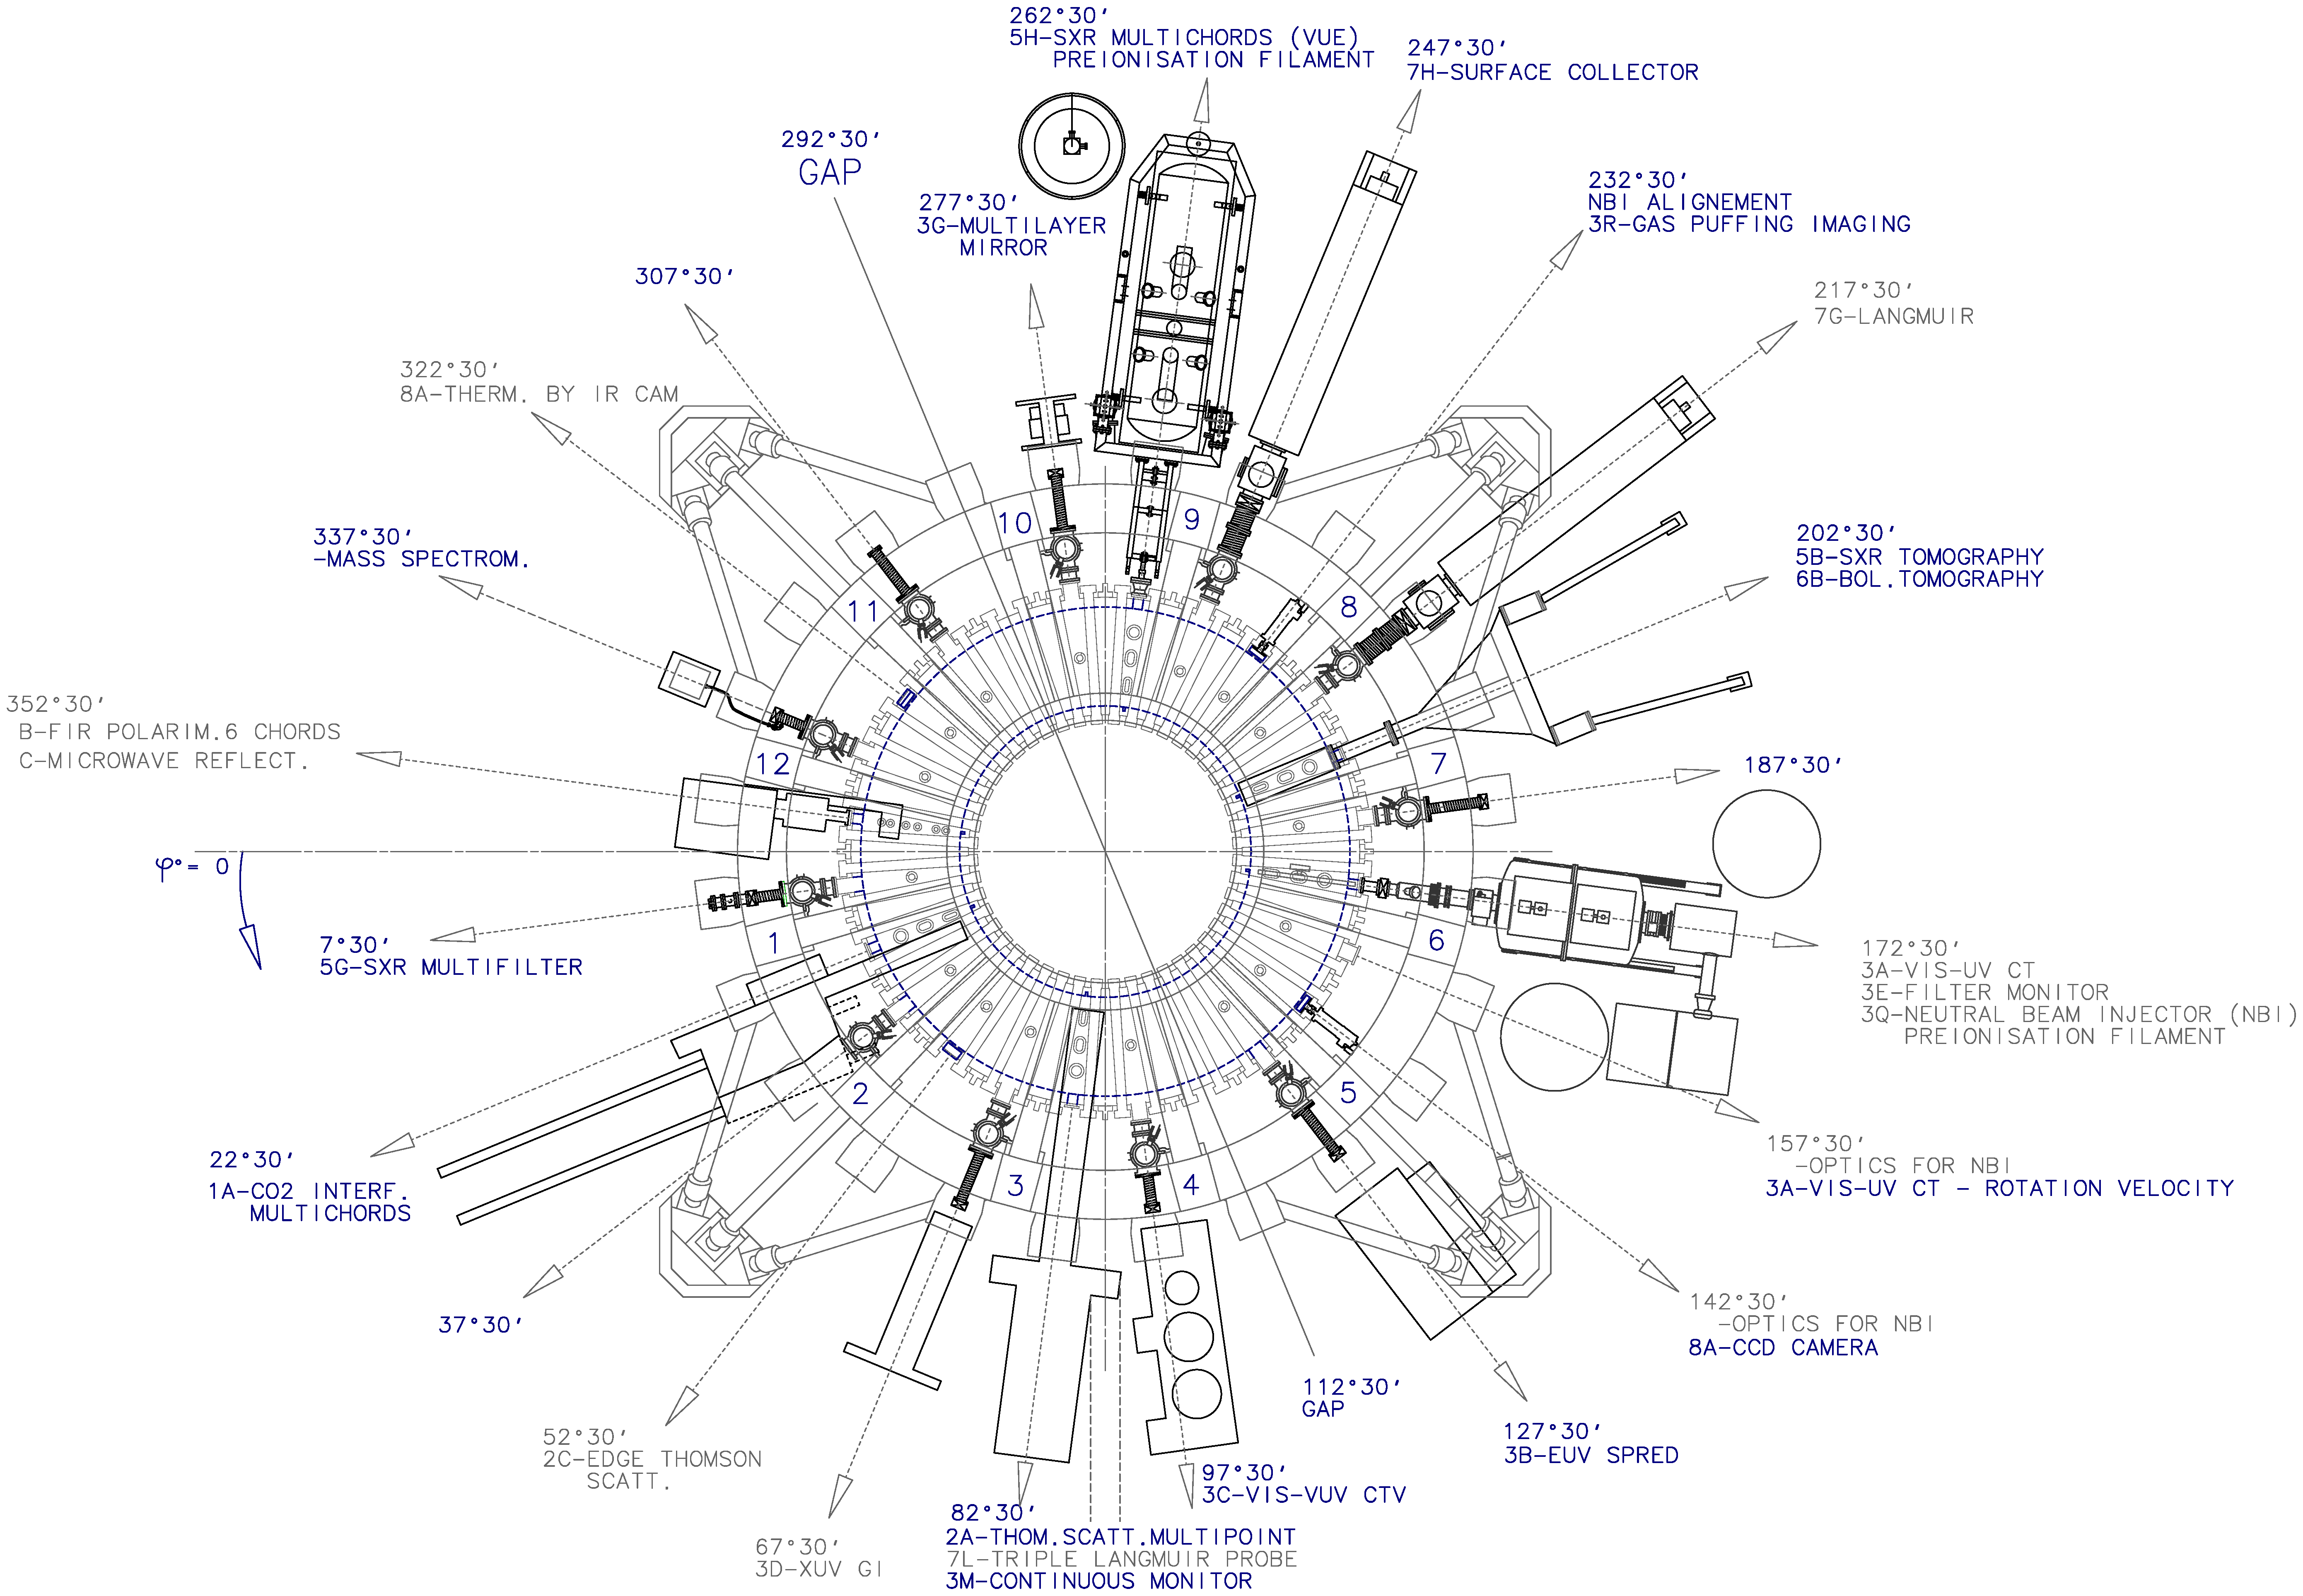
\includegraphics[width=1\textwidth]{img/rfx/Layout_Diagnosiche_AA10005.eps} \centering
% TODO: add figures
\caption{RFX map of diagnostics with related toroidal position.}
\label{rfx}
\end{figure}
%

\subsection{Thomson Scattering}
The Thomson scattering  has been a key-factor diagnostic at RFX since the initial operations for the study of RFP plasma configuration, yielding a fundamental correlation between the electron temperature diffusivity and the magnetic fluctuations that link the plasma confinement to the dynamo related modes~\cite{}. This also evolved in the possibility to identify a hot asymmetric island when the temperature gradient extends to the plasma core in the \ac{QSH} state.
During the first operation of RFX the diagnostic was composed by a single pulse of laser from ruby diode ( $\lambda = 694 nm$ ) passing through the plasma in the equatorial plane, and two grating photomultipliers spectrometers.
This apparatus presented some limitations: from the precision point of view it suffered of a poor quantum efficiency of the multialkali photocathode of the photomultiplier (MCP-PMT) resulting in a general lack of sensitivity and noisy profile at low electron temperatures. On the other hand the 20 chords acquisition that characterized the acquired plrofile with a 24 mm spatial resolution was unable to effectively investigate the details of the QSH magnetic islands.

Since the 2005 with the experiment upgrade to RFX-mod the diagnostic was completely renewed. In particular the replacement of the grating spectrometers with a set of four filter polycromators with avalance photodiodes (APD) provided a 30 times higher sensitivity and 84 points profile with a new narrow grained 7mm resolution ( $r/a$ from -0.96 to 0.84 ).
The new Nd:YLF laser diode ($\lambda=1053 nm$) located 15 m away from the center of the vacuum vessel, can produce an up to 7 J burst of 10 pulses per experiment shot. with a single light emission duration of 20ns $\ac{FWHM}$.

The light passing through plasma on the equatorial plane scatter in all directions and is collected by photomultipliers at three different windows at the end of short vertical ports. The 84 pairs of quarz fibers look all the plasma poloidal angles seen by magnifying optics located at the ports. All fibers can be also moved by a special mechanical support that can self orient during the experiment setup state; at the same time all optics can also automatically adjust focus to the desired radial position of interest.
A further side by side light path decomposes the acquired spectrum in 4 channels using a series of relay lenses.

The small amount of the solid angle covered by the acquisition, together with all this set of filters applied both at the input beam - aiming at reducing the stray light and maintaining the focus -, and at the output - for the selection of the plasma region of interest and for the decomposition of the energy spectrum - are the main reason for the required high power input.

This leads to a scattered set of acquisition pulses that are not continuously reconstructing the overall shape of plasma temperature but reduce ti a small set of usually 10 time events.

The recording systems is also quite complex: for RFX-mod the detected signal has been acquired by a modular 4-channels cPCI board dedicated for each of the spectrometers, acquiring data at 500 Msps each.

\subsection{Soft X Ray}

% We chose the most reliable and fast response diagnostics ... (SXR and Magnetic coils MHD)
% Other possible diagnostics can be added ( cope with time dim )
% Possibility to trigger in realtime other diagnostics ( i.e. Thomson Scattering )

\section{MHD}

\section{Newcomb SH}

\section{The complete “SCHEMA” from sensors to plasma parameters}
